% Adjusting chapter title format for regular (numbered) chapters
\titleformat{\chapter}[display]
  {\normalfont\huge\bfseries\centering}{\chaptertitlename\ \thechapter}{20pt}{\Huge}

% Using similar styling for unnumbered chapters but without "Chapter" prefix
\titleformat{name=\chapter,numberless}
  {\normalfont\huge\bfseries\centering}{}{0pt}{\Huge}

\titlespacing*{\chapter}{0pt}{50pt}{40pt} % Adjust vertical spacing before and after the title


\chapter{Simulations and Results} % Ensures chapter numbering starts correctly

\label{chp:4}

\section{Datasets}


\subsection{MNIST Dataset}

The MNIST dataset is a widely recognized benchmark in the field of deep neural networks (DNNs), comprising 70,000 grayscale images of handwritten digits. These images are split into 60,000 training samples and 10,000 testing samples, each of size 28x28 pixels. The dataset includes labels for each digit from 0 to 9, making it a total of 10 classes. This dataset is extensively used for evaluating the performance of various DNN algorithms due to its simplicity and the well-established baseline results it offers. To ensure the correctness our model, we selected 100 correctly classified samples from each class. This selection process involved comparing the model's predictions with the actual labels and choosing only those samples where the predictions were correct. This resulted in a balanced subset of 1,000 samples, with 100 samples from each of the 10 classes.

\subsection{DAWN Dataset}

The DAWN (Vehicle Detection in Adverse Weather Nature Dataset) dataset focuses on vehicle detection under adverse weather conditions, providing a diverse set of real-traffic images categorized into four weather conditions: fog, snow, rain, and sandstorms. Initially, the class distribution in the training set was imbalanced, with the following counts: 258 for label 1, 240 for label 0, 163 for label 3, and 160 for label 2.

To address this imbalance, we resampled the training set to ensure an equal number of samples for each class. This resulted in a balanced training set with 258 samples for each label. This balancing step was crucial for fair training and evaluation of the model, ensuring that no class was overrepresented or underrepresented.

For the testing set, we selected 100 samples from each class, ensuring a balanced evaluation dataset. This selection process was critical to accurately assess the model's performance across different classes and adverse weather conditions.




\section{Use Case 1: Handwritten Digit Recognition }
\subsection{Local Correctness Evaluation}

In this section, we evaluate the local correctness of the model under different transformations, namely rotation, noise, and brightness. Each transformation is applied with specific parameters to simulate real-world variations. Images are rotated by 25 degrees to evaluate the model's performance under rotation. Gaussian noise with a noise factor of 0.2 is added to the images to test the model's robustness to noisy conditions. The brightness of the images is increased by a factor of 0.3 to simulate different lighting conditions.

The local correctness graphs provide insights into the model's robustness under these transformations for each digit class. The model exhibited high performance under rotation (0.99) and brightness (1.00) for Class 0, with slightly reduced accuracy under noise (0.81). For Class 1, the model maintained consistently high accuracy across all transformations: rotation (0.99), noise (0.99), and brightness (1.00). However, the model struggled more with rotations (0.76) and noise (0.79) for Class 2 compared to brightness (1.00). Similarly, for Class 3, the model showed lower accuracy for rotations (0.82) and noise (0.78), but performed perfectly under brightness (1.00). 

Class 4 demonstrated high accuracy across all properties, with rotation (0.91), noise (0.86), and brightness (1.00). Class 5 maintained high performance under all transformations: rotation (0.89), noise (0.99), and brightness (1.00). The model showed noticeable difficulty with noise (0.64) for Class 6, while maintaining high accuracy for rotation (0.87) and brightness (0.99). For Class 7, high accuracy was observed under brightness (1.00), with reduced performance under rotation (0.75) and noise (0.86). The model faced significant challenges under noise (0.02) for Class 8, but maintained good performance for rotation (0.68) and brightness (0.99). Finally, for Class 9, the model showed moderate performance under noise (0.51), and high accuracy under rotation (0.93) and brightness (0.99).

Overall, the model demonstrates strong robustness to brightness changes across all classes, frequently achieving perfect accuracy. However, performance under noise is highly variable, with some classes, such as Class 8, experiencing a dramatic drop in accuracy. While the model generally handles rotations well, there remains room for improvement, particularly in addressing noise-induced challenges. This analysis highlights the necessity for targeted training to enhance the model's robustness, especially under noisy conditions for specific classes.

\begin{figure}[h]
    \centering
    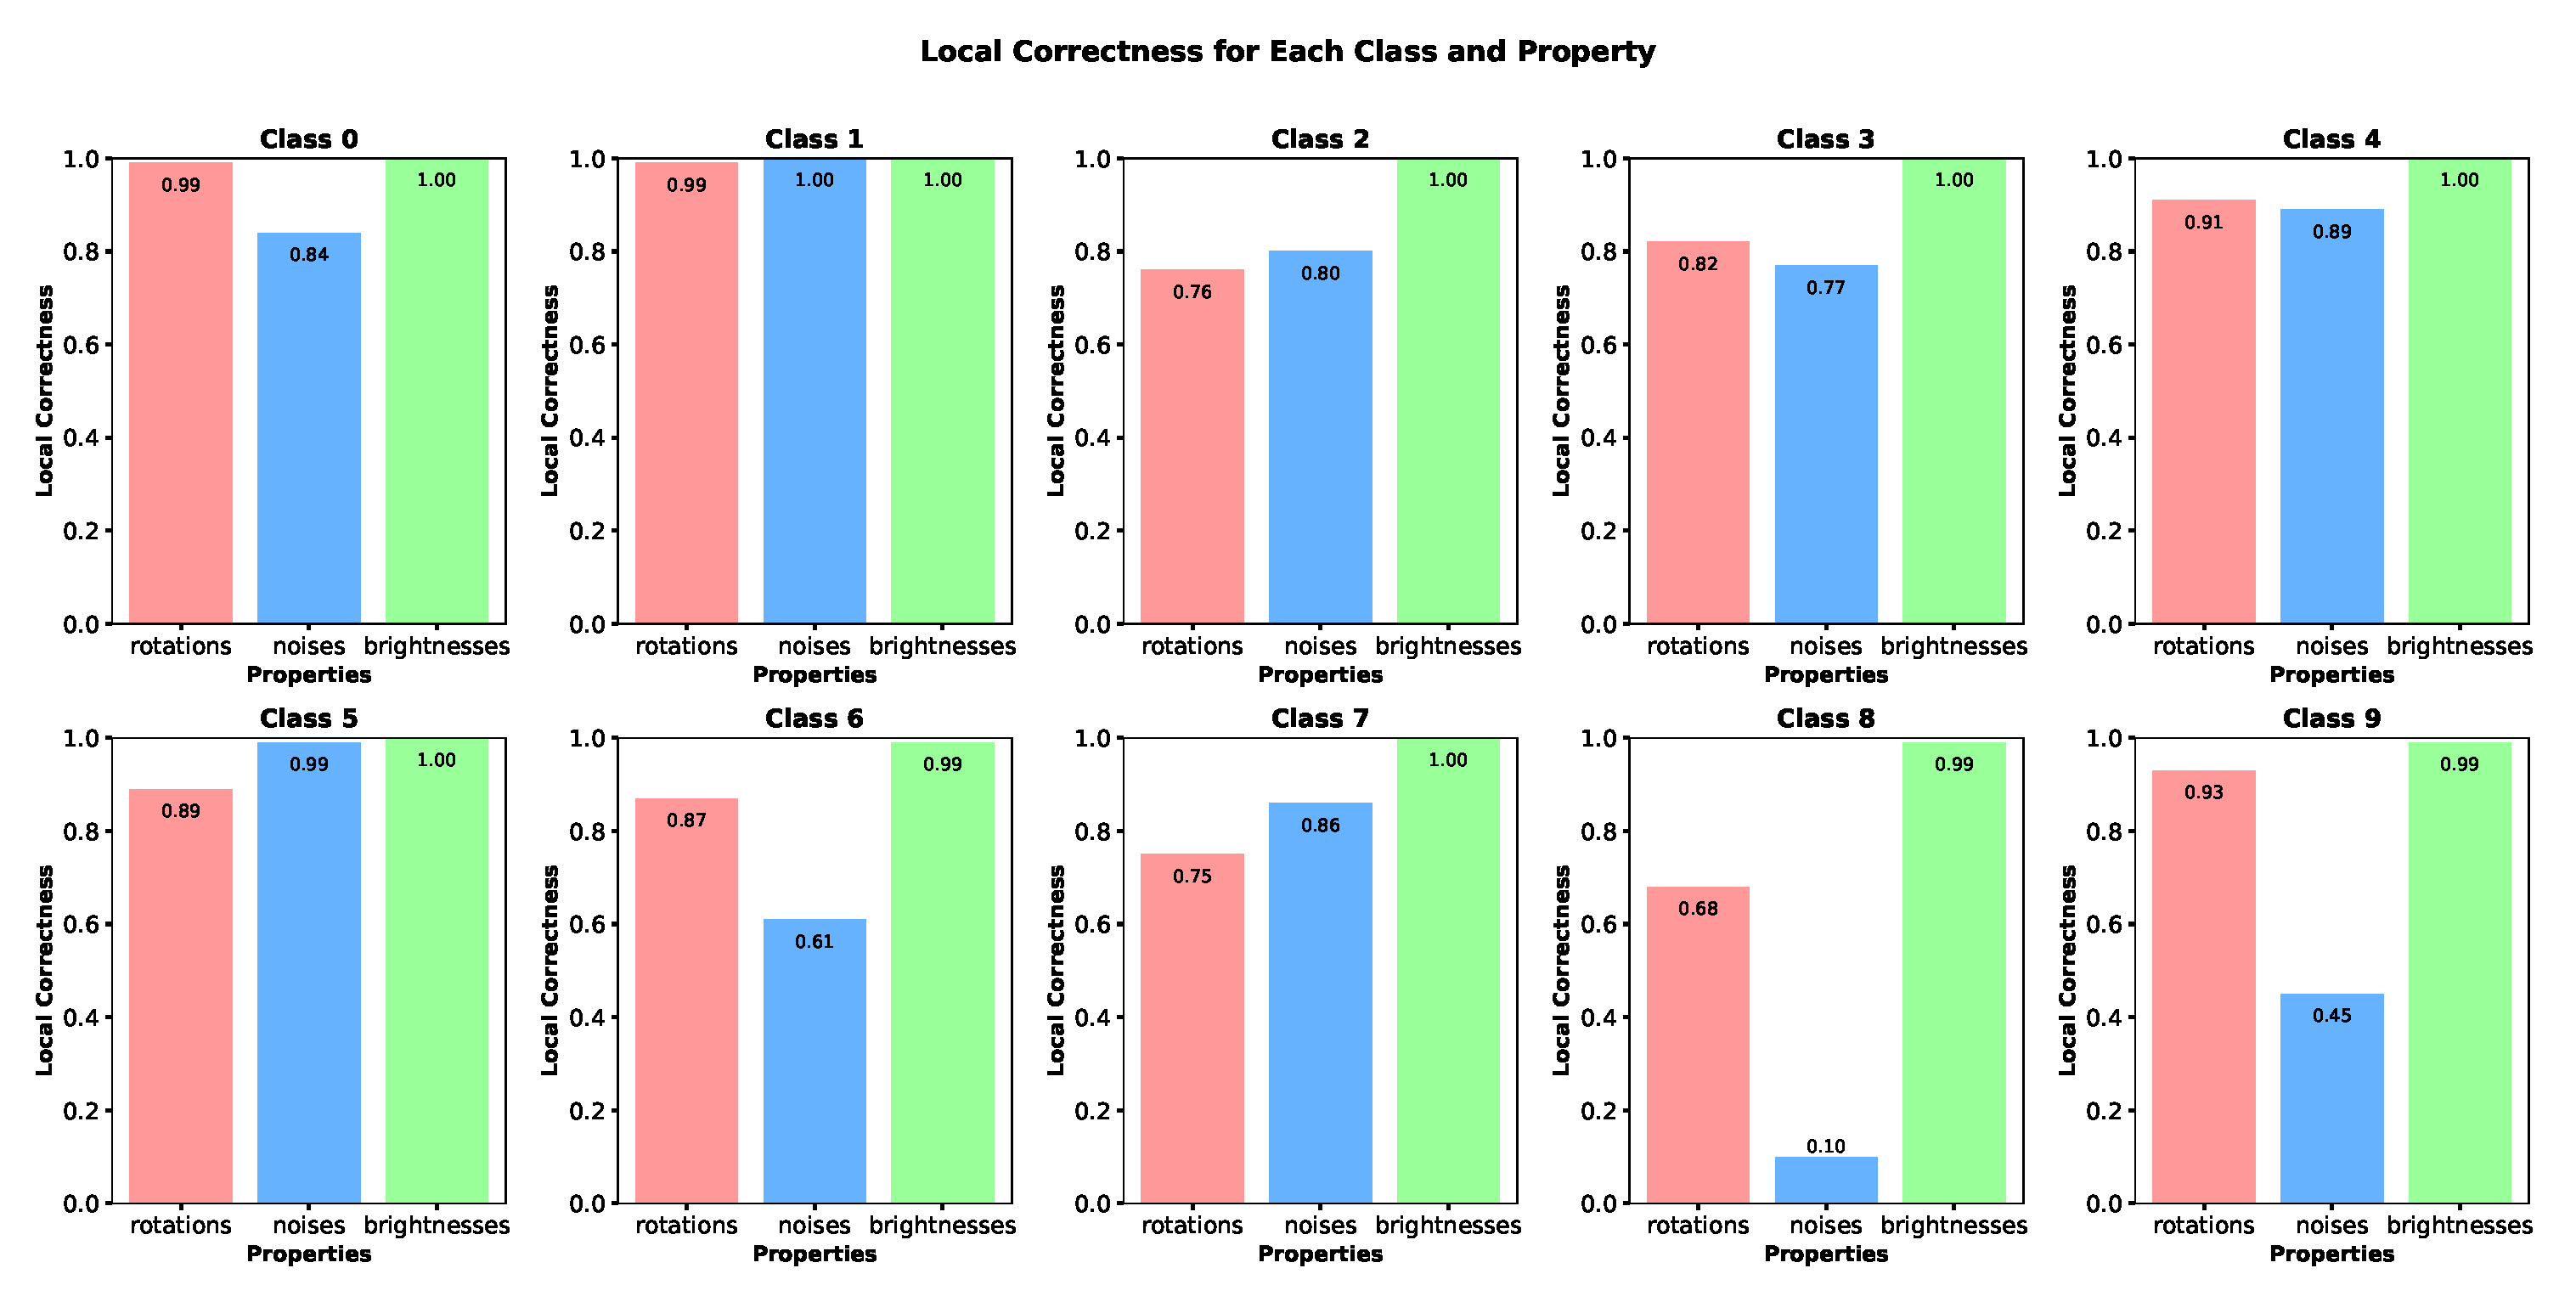
\includegraphics[width=\textwidth]{local_correctness.eps}
    \caption{Local Correctness for each Class and Property}
    \label{fig:local_correctness}
\end{figure}
\subsection{SHAP Analysis and Pixel Modification}
\begin{figure}[h]
  \centering
  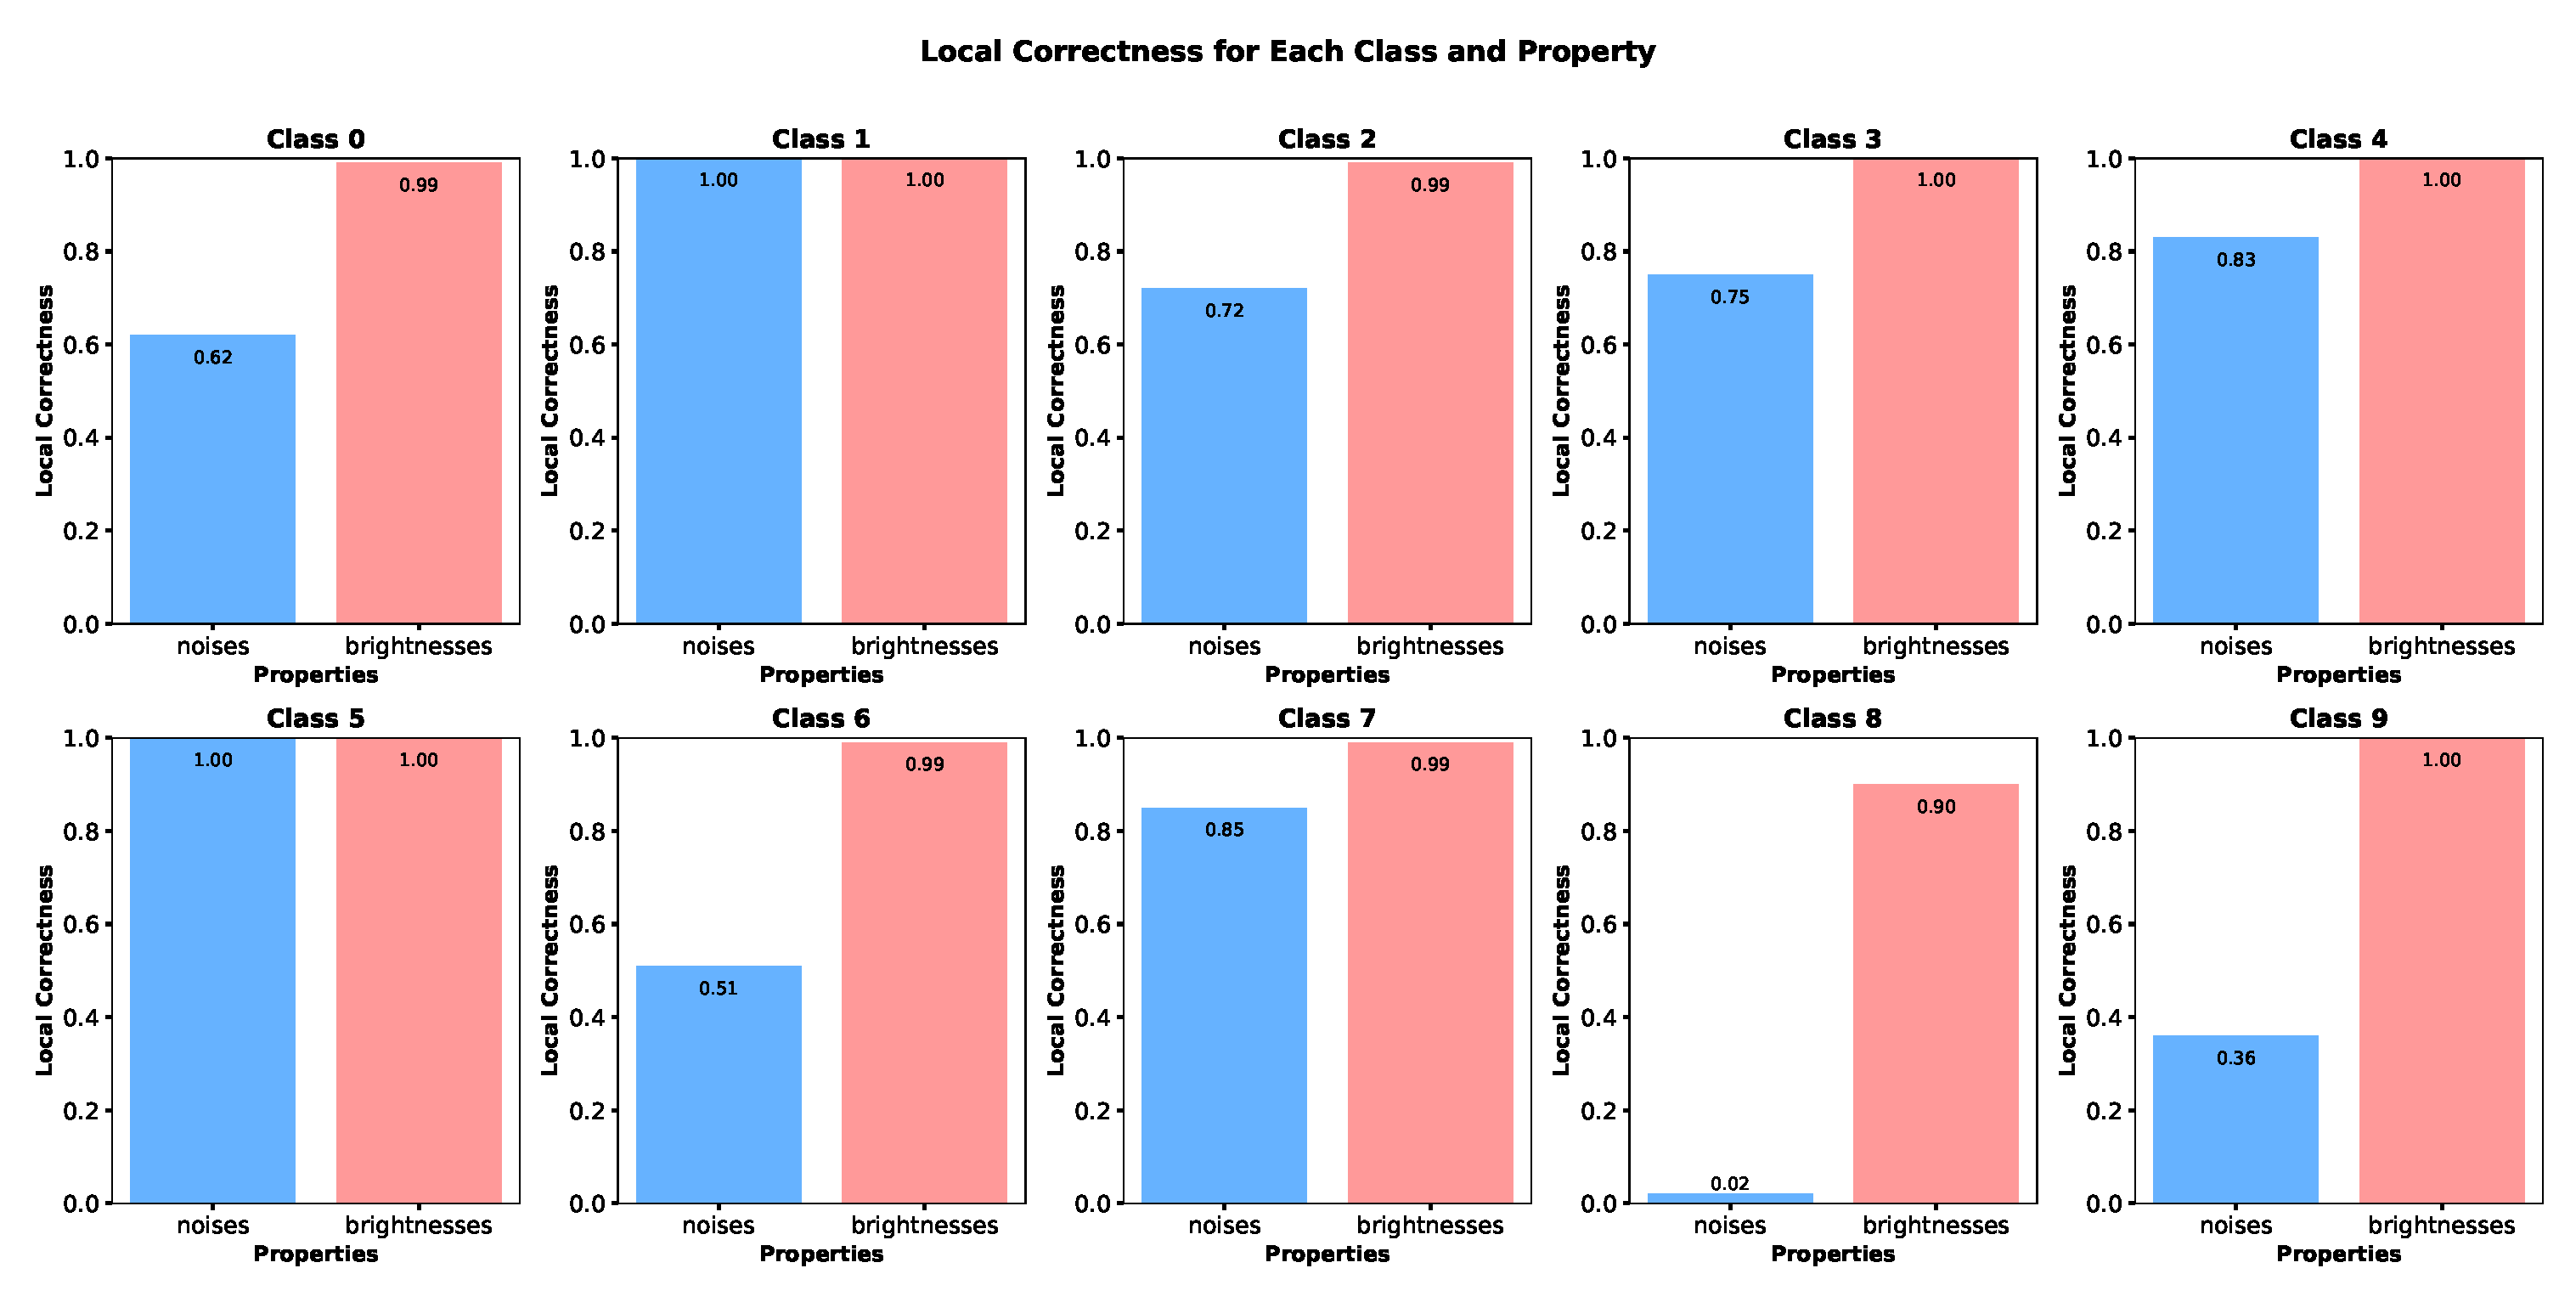
\includegraphics[width=\textwidth]{local_correctness_shap.eps}
  \caption{Local Correctness for each Class and Property based on SHAP Analysis. The bars represent the accuracy of correctly classified samples after applying noise and brightness transformations, highlighting the influence of these properties on model predictions.}
  \label{fig:local_correctness_shap}
\end{figure}

The analysis presented in Figure \ref{fig:local_correctness_shap} provides a detailed examination of the model's performance across different classes in response to noise and brightness perturbations. This evaluation was conducted following the application of SHAP (SHapley Additive exPlanations) analysis, which identified the top 30\% most influential pixels. These critical regions were then modified to simulate realistic scenarios, testing the model's robustness. The results reveal varying degrees of resilience across classes. For instance, Class 0 shows moderate robustness to noise with a correctness of 0.62, while demonstrating high robustness to brightness changes with a correctness of 0.99. Class 1, on the other hand, exhibits perfect robustness to both noise and brightness with correctness values of 1.0. Classes such as 2 and 3 maintain high robustness to brightness (0.99 and 1.0, respectively) but show a moderate decline in performance under noise. Notably, Class 8 is highly sensitive to noise, with a correctness of only 0.02, highlighting its vulnerability. Overall, brightness changes have a relatively lower impact on the model's performance compared to noise, as evidenced by consistently higher correctness values. This analysis underscores the need for targeted improvements to enhance noise robustness, particularly for classes like 6, 8, and 9, which show significant sensitivity. Addressing these weaknesses through techniques such as noise-augmented data training or more robust architectural designs will lead to a more resilient and reliable model, better suited for real-world applications where such perturbations are common.
\subsection{Global Correctness Evaluation}
The following figures illustrate the global correctness of various pairs of digits under different transformations: noise, brightness adjustment, and rotation. The final global correctness for each transformation is also depicted.

In my experiment, I checked the following specifications:

\scalebox{0.9}{%
\begin{minipage}{\linewidth}
\begin{align*}
  global\_noise &\leftrightarrow (noise\_0\_0 \land noise\_0\_1 \land noise\_0\_2 \land \ldots \land noise\_9\_9) \\
  global\_brightness &\leftrightarrow (brightness\_0\_0 \land brightness\_0\_1 \land brightness\_0\_2 \land \ldots \land brightness\_9\_9) \\
  global\_rotation &\leftrightarrow (rotation\_0\_0 \land rotation\_0\_1 \land rotation\_0\_2 \land \ldots \land rotation\_9\_9) \\
  global\_system &\leftrightarrow (global\_noise \lor global\_brightness \lor global\_rotation)
\end{align*}
\end{minipage}
}
  


\begin{figure}[H]
    \centering
    
\includegraphics[width=\textwidth]{global_correctness.eps}
    \caption{Global Correctness for Noise, Brightness, and Rotation Transformations}
    \label{fig:global_correctness}
\end{figure}

\begin{figure}[H]
    \centering
    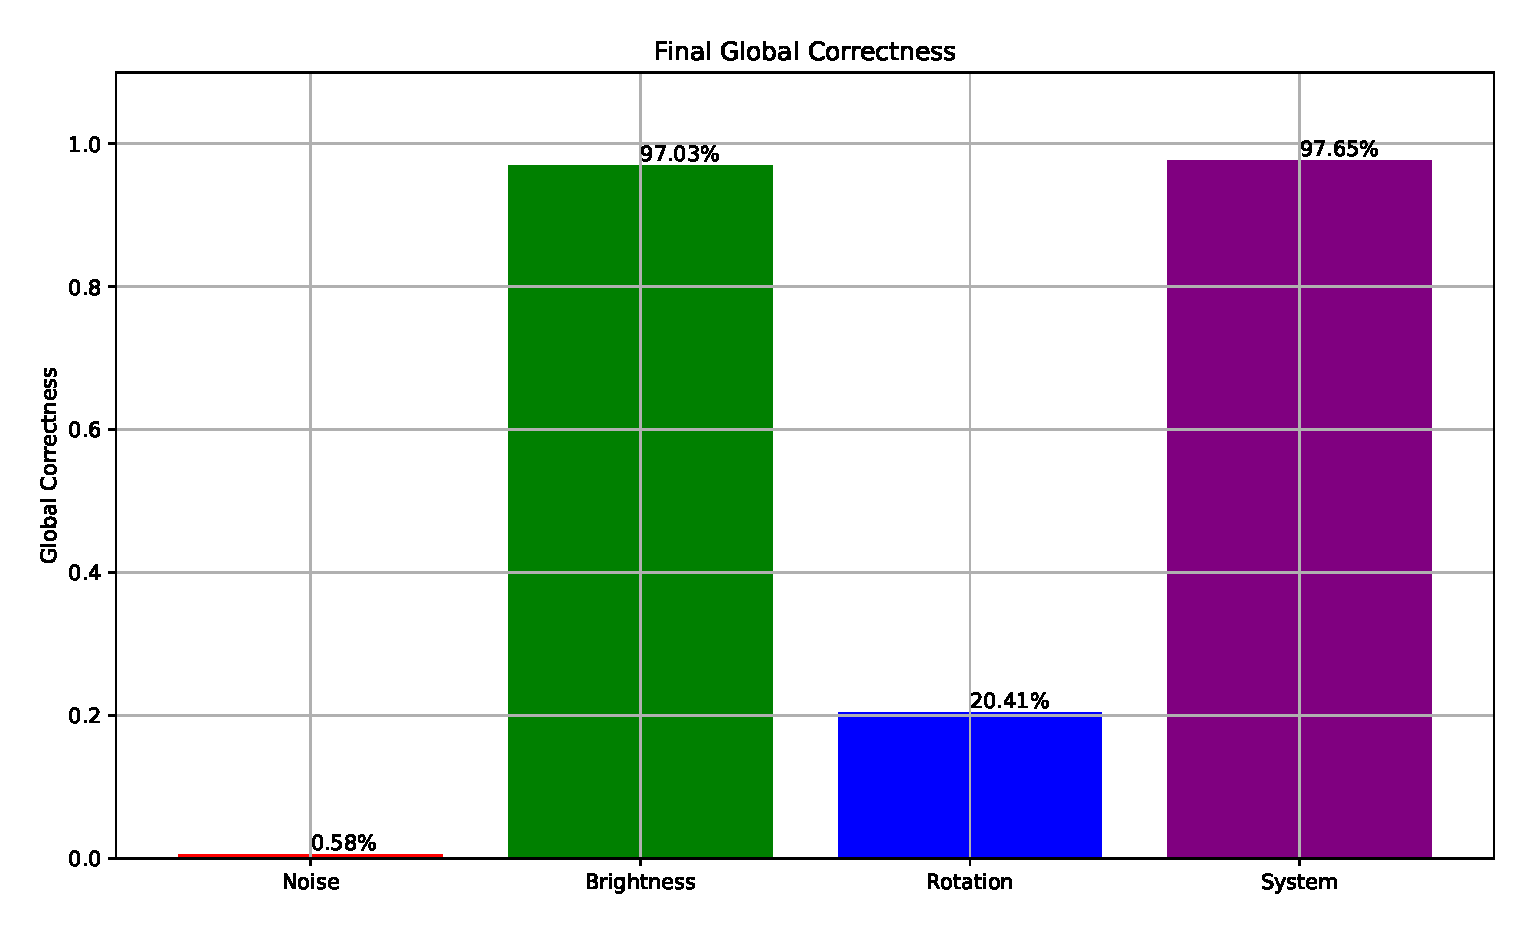
\includegraphics[width=0.8\textwidth]{global_correctness_combine.eps}
    \caption{Final Global Correctness}
    \label{fig:final_global_correctness}
\end{figure}

The global correctness values for pairs of digits under the noise transformation vary significantly. Some pairs such as (0,0), (1,1), (2,2), etc., achieve perfect correctness (100\%), while others like (0,5) and (1,8) exhibit very low correctness (3.00\% and 18.04\%, respectively). This indicates that the model's performance is highly inconsistent under noise, likely due to the distortion introduced affecting digit recognition. The model performs exceptionally well under brightness adjustments, with most pairs achieving near-perfect correctness. This suggests that the model is robust to changes in brightness, maintaining high confidence scores despite variations in image illumination. Performance under rotation is moderate, with significant variations across different pairs. Some pairs like (0,0), (1,1), (3,3), etc., achieve high correctness, while others such as (2,5) and (5,8) have lower correctness values. This variation suggests that while the model can handle certain rotations well, it struggles with others, potentially due to the angles and the inherent difficulty in recognizing rotated digits.

Combining the global correctness across all transformations, we observe an overall high performance with a final global correctness of 97.65\%. **Brightness** contributes the most to this high score (97.03\%), while Noise contributes the least (0.58\%). Rotation has a moderate impact (20.41\%), reflecting its varied performance across different pairs. These observations highlight the strengths and weaknesses of the AI subsystem under different transformations. The high performance under brightness adjustments indicates robustness to illumination changes, while the challenges with noise and rotation suggest areas for improvement in handling these perturbations.
\subsection{Analysis of Global Correctness After SHAP Analysis}
The analysis of the global correctness graphs for noise transformations, both with and without SHAP analysis, clearly shows the importance of using SHAP to find key areas in the data. 

In the first graph, which looks at individual noise pairs, supports this finding by consistently showing lower correctness for each pair when SHAP analysis is used. The pattern of reduced performance across different pairs indicates that SHAP is effective at identifying critical parts of the data that, when altered, reveal the model's weaknesses.

The second graph, we see that the global correctness for noise transformations drops dramatically from 58\% without SHAP to just 0.25\% with SHAP. This significant drop suggests that when the most important pixels identified by SHAP are changed, the model's performance suffers greatly. This is important because it helps us find areas where the model is weakest against noise.

These results demonstrate that using SHAP to create test cases by focusing on important pixels is a powerful method for discovering counterexamples. By systematically changing these key areas, we can stress-test the model and uncover its limitations under noisy conditions. This approach not only highlights where the model currently struggles but also points to ways we can improve its robustness. By addressing these weaknesses, we can build more reliable models that perform well even when there is noise in the data.
% The analysis of global correctness following the application of SHAP (SHapley Additive exPlanations) values provides critical insights into the model's performance under different conditions. The SHAP values, which identified the top 30\% most influential pixels, were used to modify the test samples and assess the impact on model performance. The results highlight significant disparities in the model's robustness to noise and brightness. The global correctness for noise is alarmingly low at 0.25\%, indicating a severe sensitivity to noise modifications. This suggests that the model's ability to correctly classify images drastically diminishes when noise is introduced, pointing to a critical weakness that needs to be addressed. Conversely, the global correctness for brightness stands at a robust 83.77\%, showcasing the model's resilience to changes in brightness. This high performance under brightness modifications suggests that the model has effectively learned the key features that remain invariant to lighting conditions. Overall, the system's correctness is 85.51\%, reflecting the combined effect of noise and brightness, where the robustness to brightness significantly bolsters the overall performance despite the poor noise resilience. Detailed analysis of class pair correctness further underscores this variability, with some pairs achieving 100\% correctness under noise and others plummeting to 4\%. In contrast, correctness under brightness remains consistently high across class pairs. This critical analysis reveals that while the model is robust to brightness changes, there is a significant vulnerability to noise that must be mitigated. Future efforts should focus on enhancing noise robustness, potentially through noise augmentation during training, to improve the model's overall reliability and performance in diverse real-world conditions.
% \begin{figure}[H]
%   \centering
%   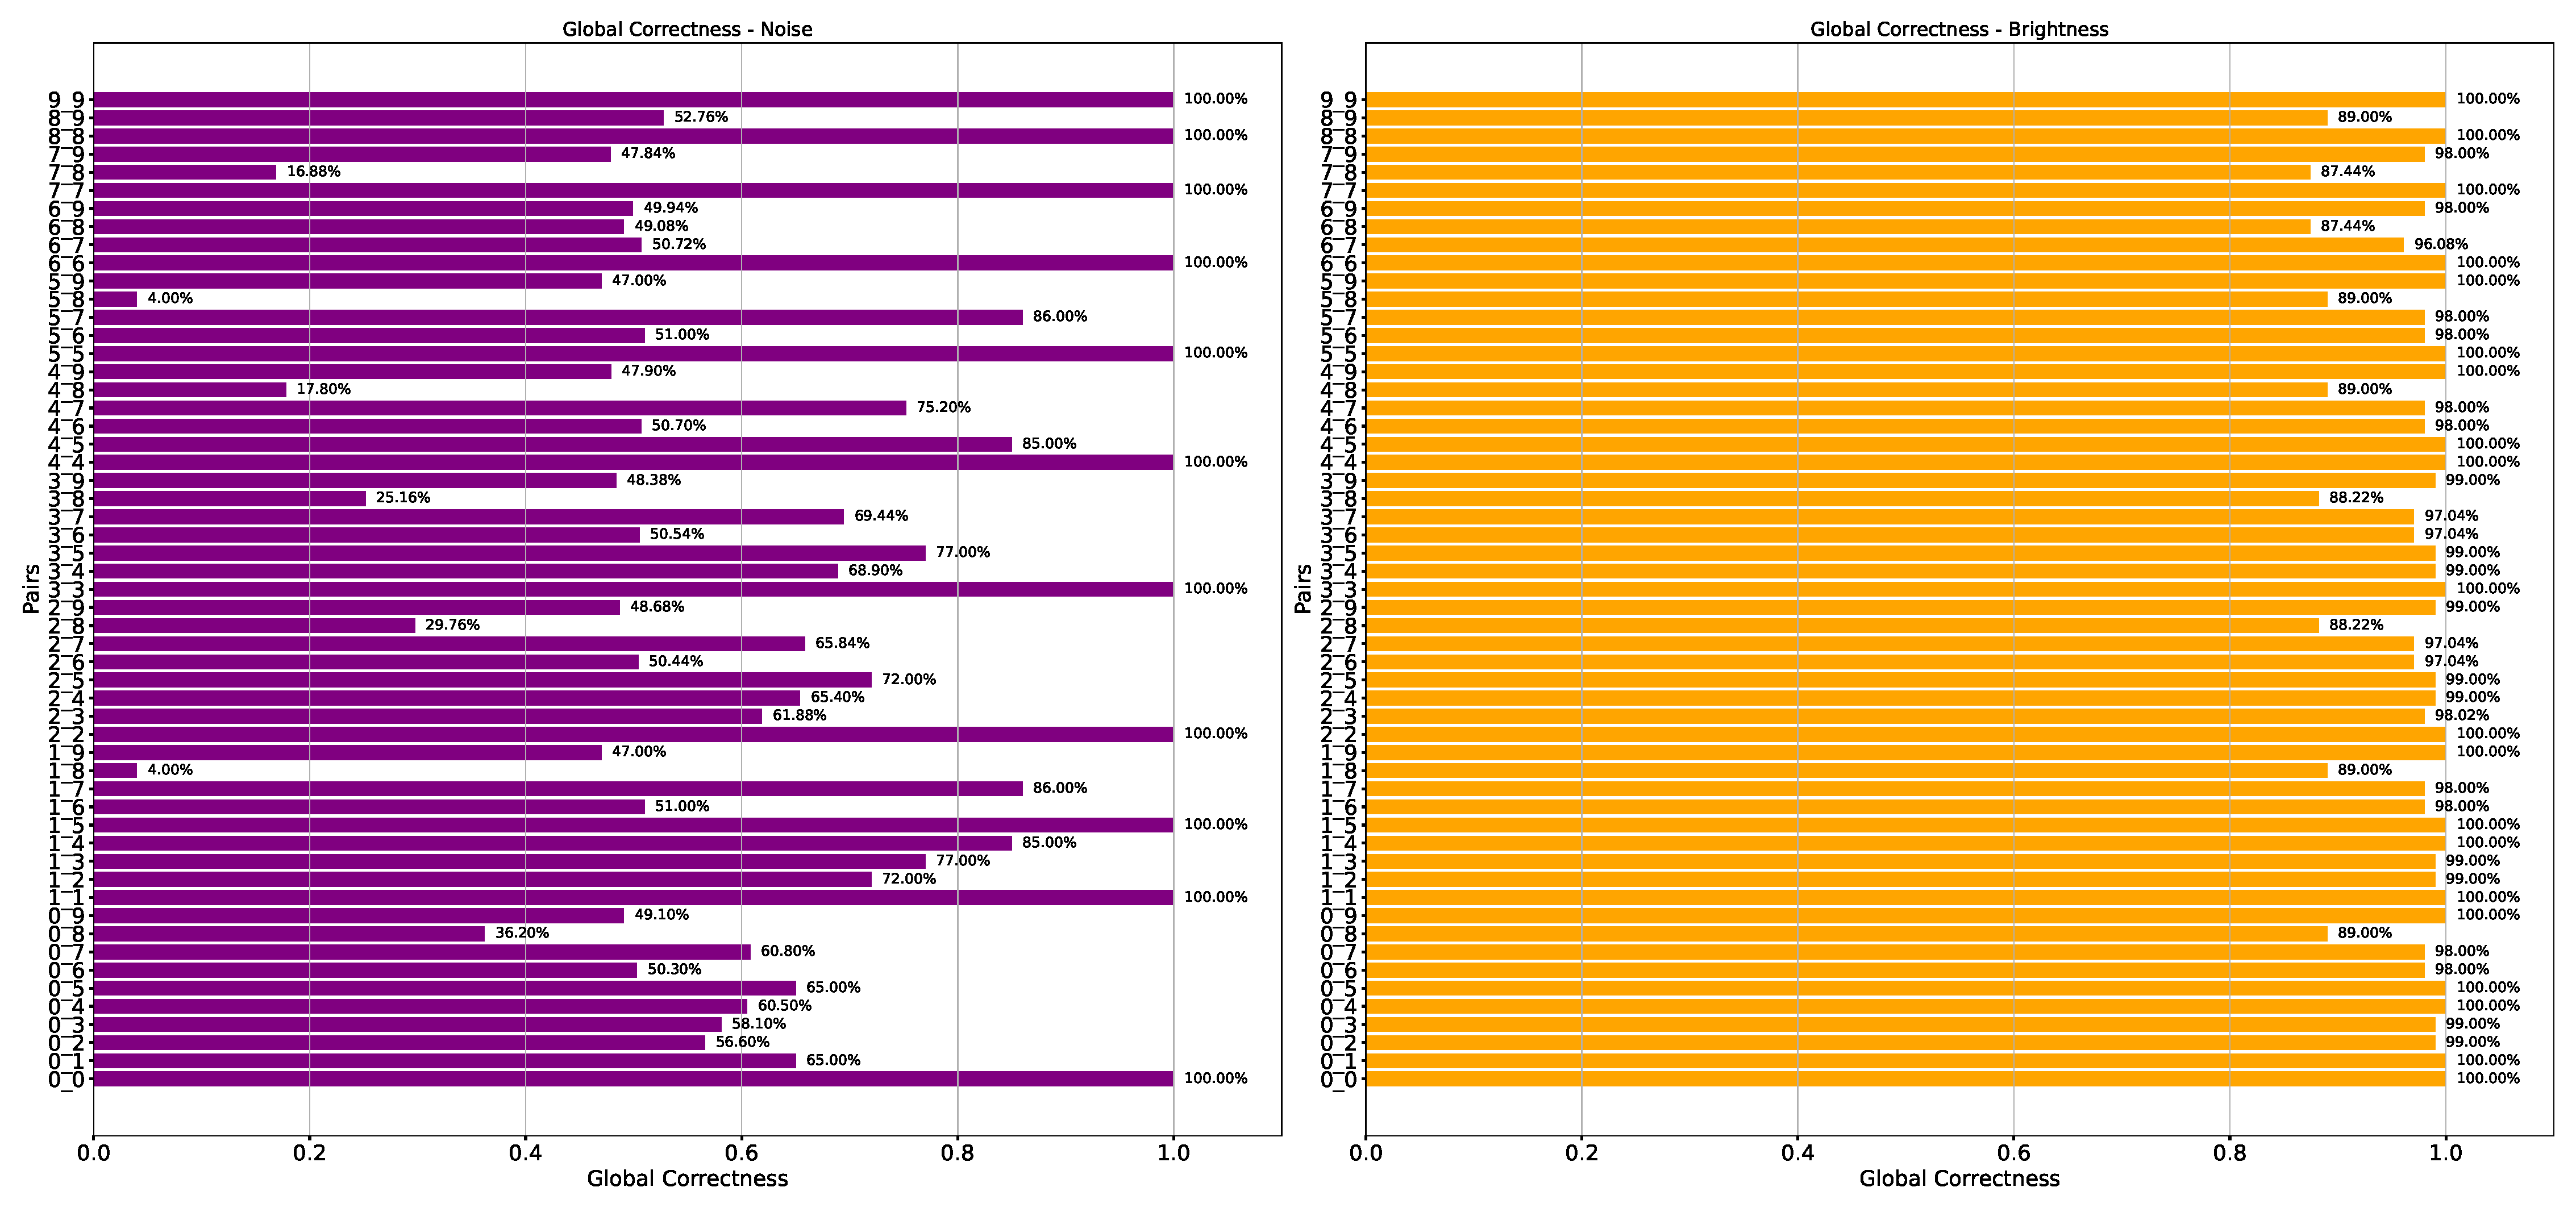
\includegraphics[width=\textwidth]{global_correctness_shap.eps}
%   \caption{Global Correctness for Noise and Brightness Transformations}
%   \label{fig:global_correctness}
% \end{figure}

% \begin{figure}[H]
%   \centering
%   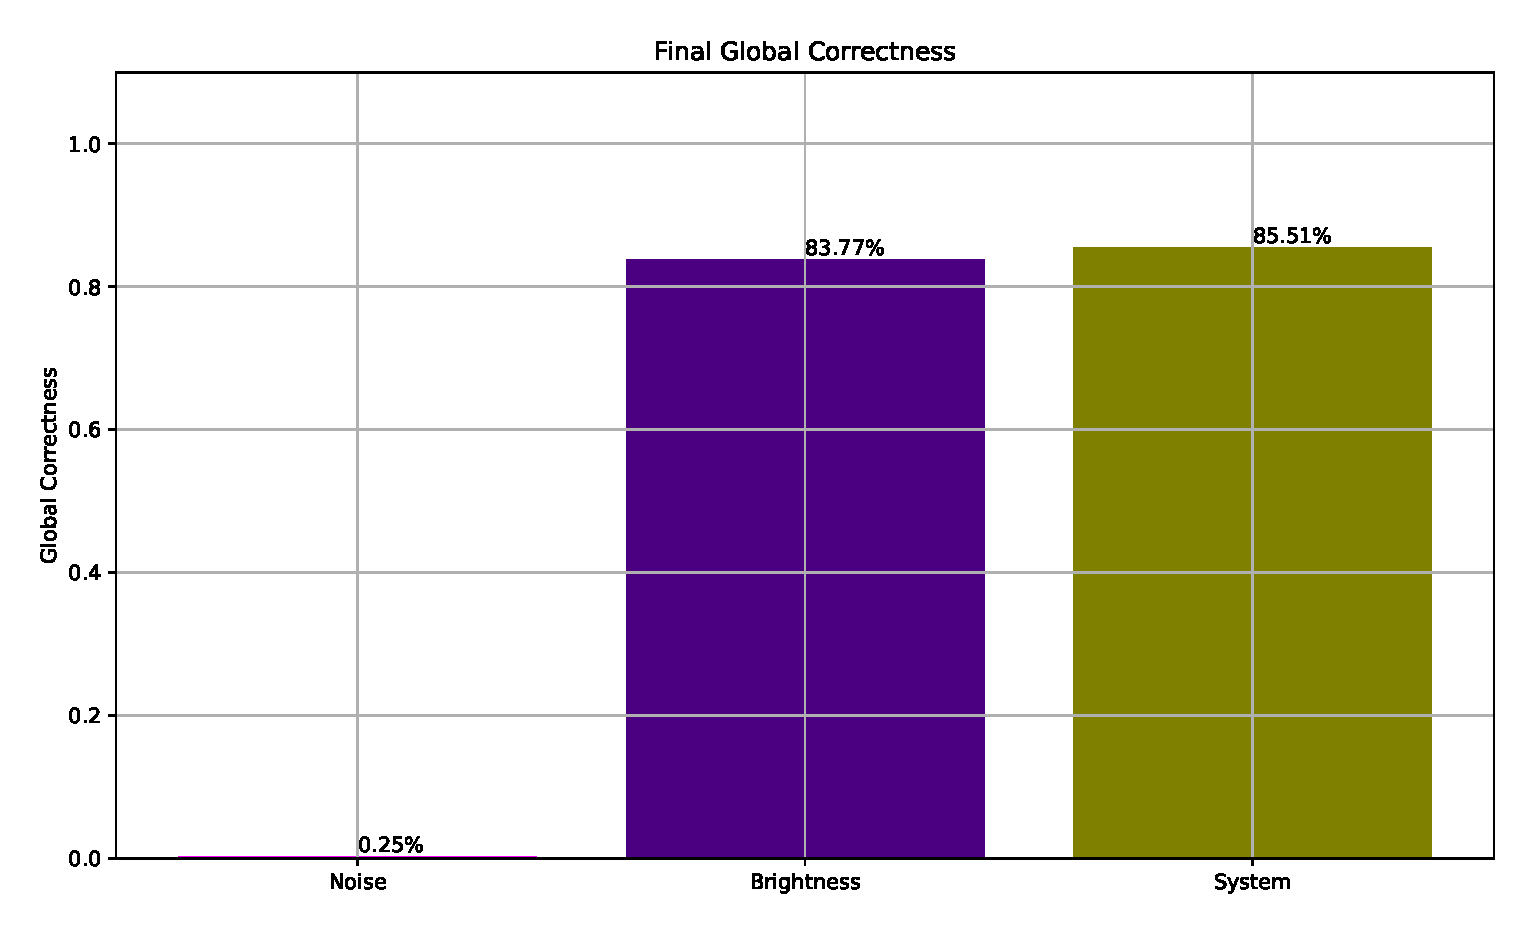
\includegraphics[width=0.8\textwidth]{global_correctness_combine_shap.eps}
%   \caption{Final Global Correctness}
%   \label{fig:final_global_correctness}
% \end{figure}

\begin{figure}[H]
  \centering
  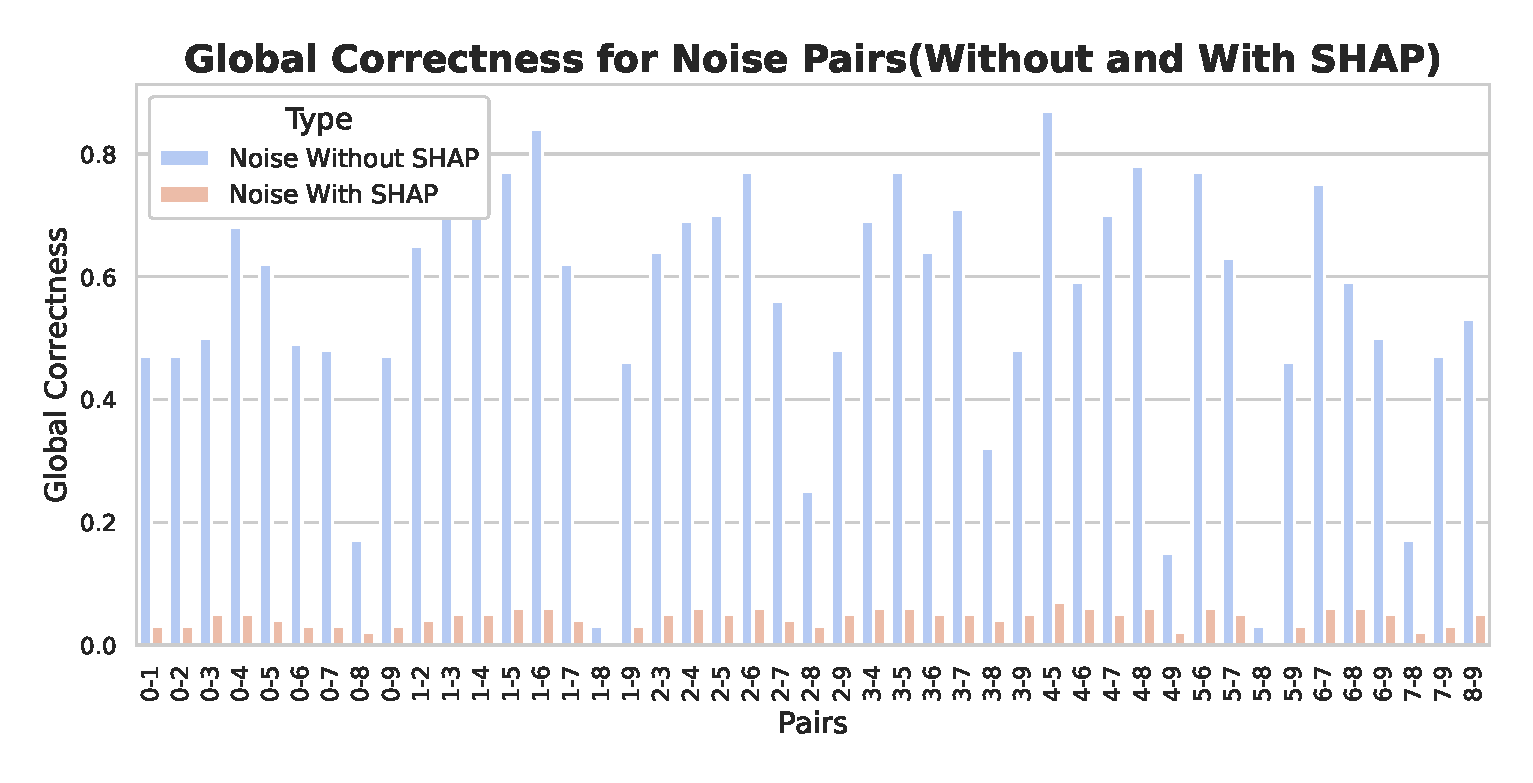
\includegraphics[width=0.99\textwidth]{global_correctness_noise_comparison.eps}
  \caption{Global Correctness for Noise pairs}
  \label{fig:global_correctness_noise_shap}
\end{figure}


\begin{figure}[H]
  \centering
  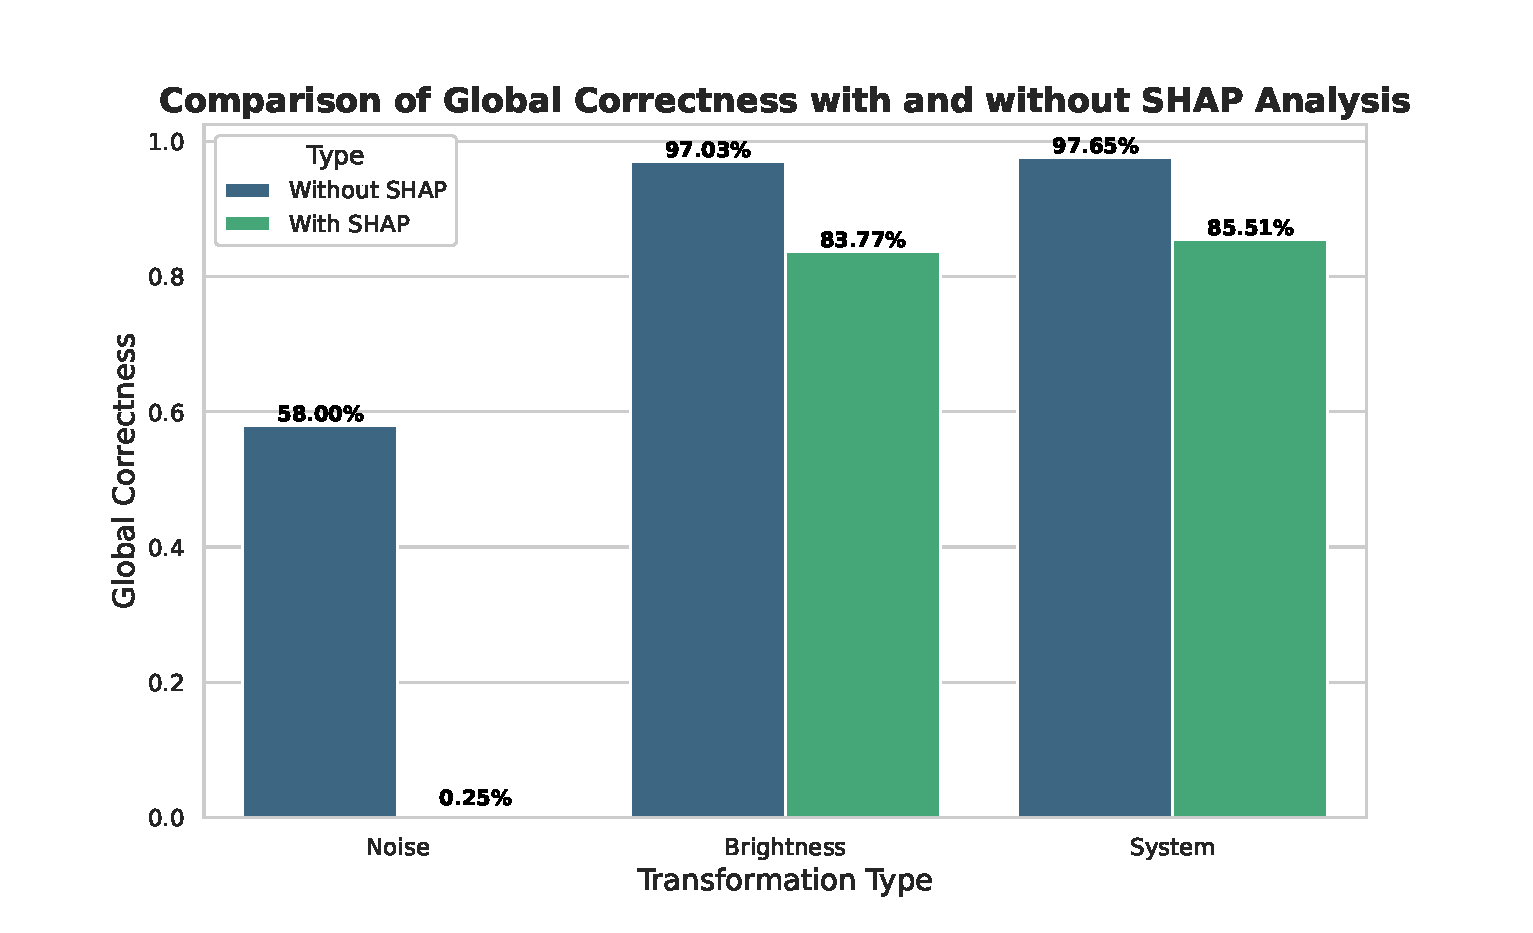
\includegraphics[width=0.8\textwidth]{combined_global_correctness.eps}
  \caption{Combine Global Correctness}
  \label{fig:combine_global_correctness}
\end{figure}
\section{Use Case 2: Autonomous Vehicle Perception}

In this use case, we investigate the robustness of an AI system for autonomous vehicles in detecting objects, particularly vehicles, under various weather conditions including fog, rain, snow, and sand. The goal is to assess the system's performance across these challenging environments to ensure reliable operation.

The dataset was split into training and validation sets, with class balancing performed through oversampling to address any class imbalances. Data augmentation techniques such as rotation, width and height shifts, shear transformation, zoom, and horizontal flips were applied to the training set to enhance the model's generalizability.

The trained model's performance was evaluated on a balanced validation set resampled to ensure uniform class distribution.

\subsection{Local Correctness Analysis}

The local correctness of the model for each weather condition is depicted in the first graph. The AI system exhibits the following correctness values:
- \textbf{Fog:} The detection correctness is 51\%, indicating moderate performance. Fog conditions likely introduce significant visual obstructions that challenge the model's ability to correctly identify vehicles.
- \textbf{Rain:} Achieving a correctness of 75\%, the model performs relatively well in rainy conditions, suggesting robustness to moderate visual disturbances caused by rain.
- \textbf{Snow:} Similar to rain, the system shows a correctness of 75\%, demonstrating its capability to handle snowy environments, where the visual contrast might be reduced.
- \textbf{Sand:} With the highest correctness of 88\%, the model excels in sandy conditions, possibly due to clearer visibility compared to other adverse weather scenarios.

\subsection{Global Correctness Analysis}

The second graph illustrates the global correctness for vehicle detection under different combination methods of weather conditions:

\scalebox{0.9}{%
\begin{minipage}{\linewidth}
\begin{align*}
  global\_weather &\leftrightarrow (fog \land rain \land snow \land sand) \\
  global\_weather &\leftrightarrow (fog \lor rain \lor snow \lor sand) \\
  global\_weather &\leftrightarrow (fog \land (rain \lor snow \lor sand))
\end{align*}
\end{minipage}
}

\begin{figure}[h]
  \centering
  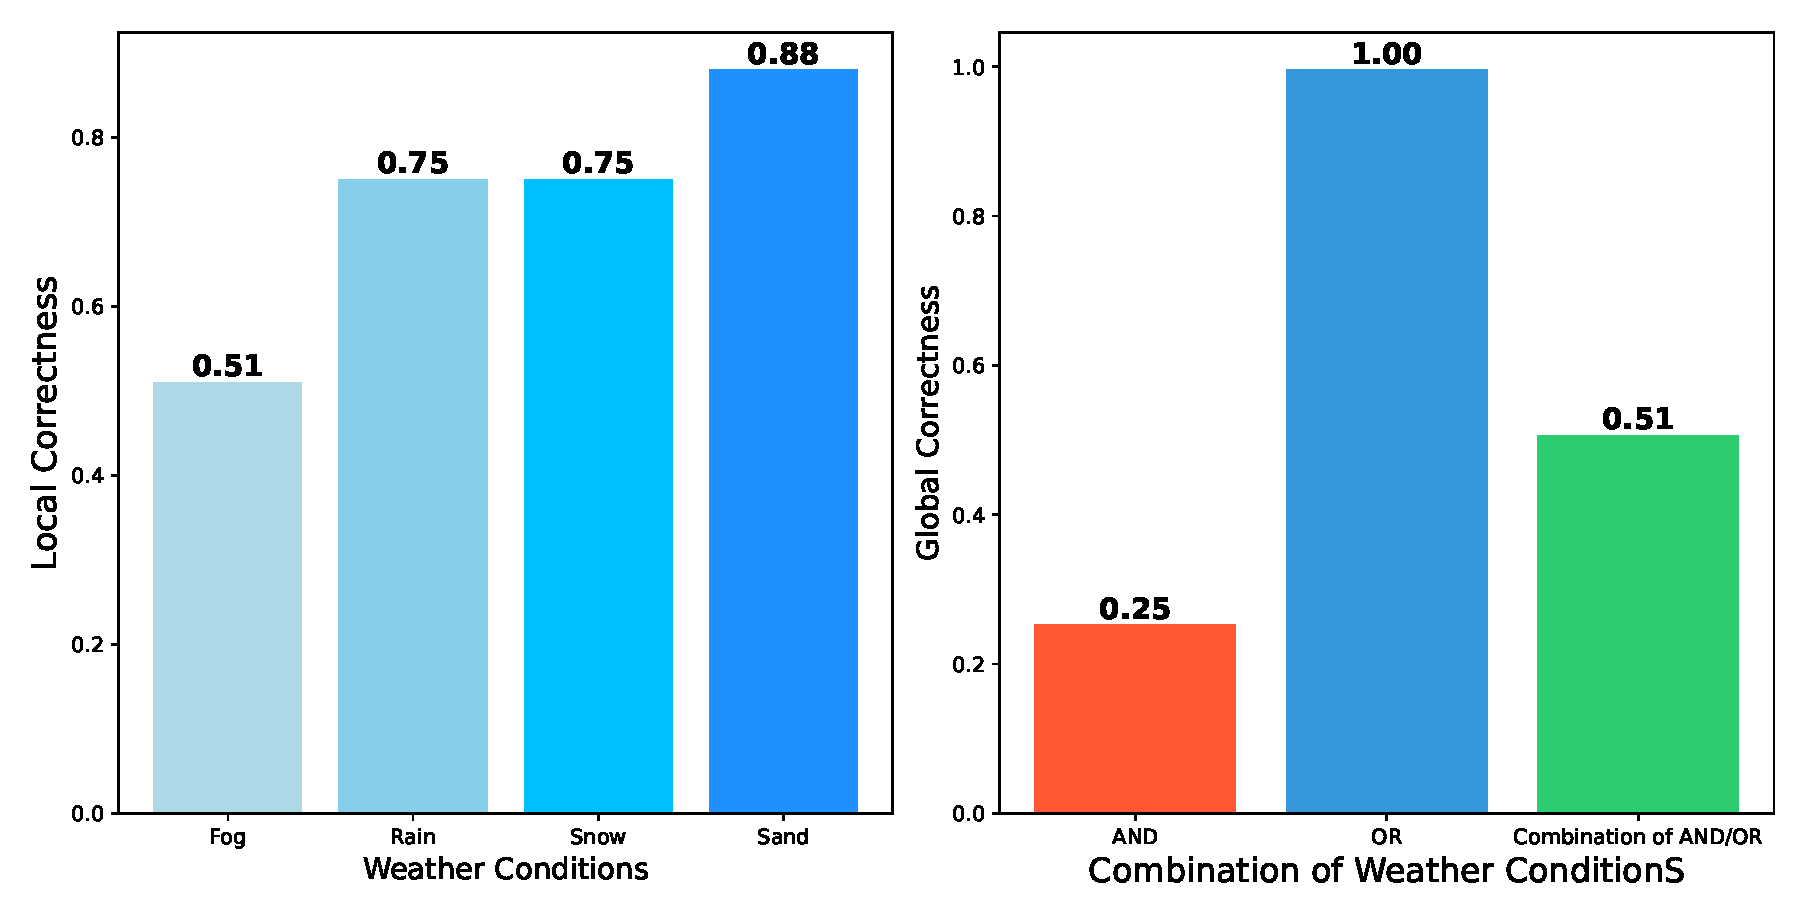
\includegraphics[width=0.8\textwidth]{globalcorrectness_vehicle_detection.eps}
  \caption{Local and Global Correctness of Vehicle Detection Under Various Weather Conditions}
  \label{fig:global_correctness_vehicle_detection}
\end{figure}




\begin{itemize}
    \item \textbf{AND (Intersection):} The model's correctness is 25\%. This low value reflects the stringent requirement for the system to correctly detect vehicles under all specified conditions simultaneously, highlighting potential vulnerabilities when multiple weather challenges are present.
    \item \textbf{OR (Union):} Achieving a perfect correctness of 100\%, the model successfully detects vehicles under at least one of the conditions. This high performance underscores the system's reliability when at least one favorable condition is present.
    \item \textbf{Combination of AND/OR:} The correctness stands at 51\%, representing a balanced approach where the model must correctly detect vehicles under fog and any one of the other conditions (rain, snow, or sand). This mixed strategy provides a realistic measure of the system's robustness in practical scenarios with varying weather conditions.
\end{itemize}



\newpage

%results
